% !TEX TS-program = pdflatex
% !TEX encoding = UTF-8 Unicode

% This is a simple template for a LaTeX document using the "article" class.
% See "book", "report", "letter" for other types of document.

\documentclass[12pt]{article} % use larger type; default would be 10pt

\usepackage[utf8]{inputenc}

%%% PAGE DIMENSIONS
\usepackage{geometry} % to change the page dimensions
\geometry{a4paper} % or letterpaper (US) or a5paper or....
% \geometry{margin=2in} % for example, change the margins to 2 inches all round
% \geometry{landscape} % set up the page for landscape
%   read geometry.pdf for detailed page layout information

\usepackage{graphicx} % support the \includegraphics command and options

% \usepackage[parfill]{parskip} % Activate to begin paragraphs with an empty line rather than an indent

%%% PACKAGES
\usepackage{fullpage}
\usepackage{amsmath,amsfonts,amssymb,proof}
\usepackage{url,hyperref}
\usepackage{wasysym}

\usepackage[boxed,commentsnumbered]{algorithm2e}
\usepackage[numbers]{natbib}

\usepackage{booktabs} % for much better looking tables
\usepackage{array} % for better arrays (eg matrices) in maths
\usepackage{paralist} % very flexible & customisable lists (eg. enumerate/itemize, etc.)
\usepackage{verbatim} % adds environment for commenting out blocks of text & for better verbatim
\usepackage{subfig} % make it possible to include more than one captioned figure/table in a single float
% These packages are all incorporated in the memoir class to one degree or another...

%%% HEADERS & FOOTERS
\usepackage{fancyhdr} % This should be set AFTER setting up the page geometry
\pagestyle{fancy} % options: empty , plain , fancy
\renewcommand{\headrulewidth}{0pt} % customise the layout...
\lhead{}\chead{}\rhead{}
\lfoot{}\cfoot{\thepage}\rfoot{}

%%% SECTION TITLE APPEARANCE
\usepackage{sectsty}
\allsectionsfont{\sffamily\mdseries\upshape} % (See the fntguide.pdf for font help)



\title{\textit{explotiv}: a phylogenetically-inspired de novo transcriptome explorer}
\author{Camille Scott}


\begin{document}
\maketitle

\section{Introduction}

As next-generation sequencing technology has become increasingly cheap and accessible, many labs are opting to use sequencing for their projects. For groups looking to quickly and cheaply produce a working profile of genes in an organism, RNA-seq has become a favored method. An RNA-seq experiment produces hundreds of millions of short sequence fragments, "reads," from the transcribed RNA of an organism. A variety of methods, one of them de novo assembly, is used to weave together these short reads
and build an approximation of the transcripts which existed in the donor organism. These transcripts would eventually be translated
 into proteins, meaning that their sequence content and abundances are valuable to the understanding of the function of an organism.
 Characterizing a set of transcripts (a transcriptome) is a continuing field of research: actually assembling the reads into full length
 transcripts, estimating the expression level of those transcripts, and annotating them by identifying the names, structure, and function
 of those transcripts being major topics. While significant progress has been made in all these pursuits, a key item missing is the ability to
 rapidly summarize and compare entire transcriptomes. With many studies being published every day with newly assembled and annotated transcriptomes, this absence becomes more clear.
 
 This paper introduces \textit{explotiv}, a visualization tool for summary exploration of annotated transcriptomes. The \textit{explotiv}
 visualization method is inspired by traditional phylogenetic analyses, producing summary plots of transcriptomes in a format
 which is digestible by biologists. The use of modern visualization tools allows the results to be explored in the browser, interactively,
 as well as exported to be integrated in to publications.

\section{Background}

While several tools make efforts to quantitatively assess de novo assembled transcriptomes, these are mostly focused on assessing
the assembled sequence content relative to the reads which produced them: that is, they assess the assembly software's ability
to faithfully construct transcripts from reads. While this is certainly a useful and necessary tool for anyone working with de novo
transcriptome assembly, it does not necessarily inform the user whether the reads themselves are poorly sampled, whether
there is contamination, or even more broadly, whether the assembled transcripts can be appropriately annotated. Further,
these tools mostly generate static plots for individual data dimensions (such as "percentage of reads mapped per sample"), or
simply output tables and no plots at all. 

When it comes to visualizing annotation results, the situation is even more grim. Most publications include tables with the number
of proteins, protein domains, or genes matched in a given database, and/or Venn diagrams showing matched proteins fitting certain
criteria; these methods, while they convey useful information, are poor at providing biological context. \textit{explotiv} addresses
this problem by putting evolutionary context squarely in the center: we view the transcriptome through the lens of its similarity
to extant clades, rather than a pile of transcripts with database similarities.

\section{Methods}

\subsection{Protein Mapping}

The first step is to produce a mapping from transcript to known proteins. This is accomplished efficiently using LAST 
for translated DNA to protein alignment \cite{kielbasa_adaptive_2011} \cite{sheetlin_frameshift_2014}. The
explotiv prototype uses OrthoDB version 8 \cite{waterhouse_orthodb:_2011} as its reference protein database, due
to its manageable size, lack of redundancy, and vetted ortholog groups. LAST produces a one one-to-many mapping
from the transcript database to the protein database; we use all alignments from each transcript, filtering out any
with expectation-value (e-value) below $.000001$ to remove alignments that have a high probability of being
false positives.

\subsection{Tree Building}

\subsubsection{Base Tree}

\textit{explotiv} builds its summary visualization on a base phylogenetic tree, which was generated from the NCBI Taxonomy Database
\cite{sayers_database_2009}. The base tree is the tree induced by the set of species represented in the OrthoDB
database; OrthoDB contains proteins from 400 model organisms, which induces a tree of ~1200 total nodes. 
This base tree contains organisms from the fungi and the metazoans; OrthoDB does not include any prokaryotes,
so the current base tree does not include them either. This tree is output as a JSON file suitable for consumption 
in most programming languages.

An important caveat is that the NCBI Taxonomy Database does not represent a true phylogeny: as might be inferred 
from the name, it is a taxonomy, where groupings are not always informed by evolutionary relationships.
Further, and perhaps more importantly, it lacks branch lengths, which are a basic piece of information for all phylogenetic
trees. To help overcome this limitation, we simply assume each branch to have length 1; however, future versions
will need to use more phylogenetically accurate trees.

\subsubsection{Calculating Node Scores}

The bulk of the visualization generation is in calculating scores for each node in the tree based on the protein alignments.
Our initial set of alignments map only to the leaf nodes in the tree, but the goal of the method is to assign scores
to all clades. We must design an algorithm to propagate these scores up the tree in a way that is phylogenetically sound.
Our method is sketched out for a single transcript $s \in S$ like so: take the collection of alignments $a_s \in A$ for the transcript 
and their corresponding species identifiers. Then, use the identifiers to map each alignment score to its corresponding leaf
node, with all non-mapped leaf nodes from the tree $T$ receiving scores of 0. We can then propagate the scores up the tree recursively, 
scoring each internal node as the sum of its descendants' scores divided by the sum of the branch lengths in its descendants' subtree. This process is repeated for every transcript, resulting in an $|S| \times |T|$ score matrix $M_s$ of scores. The final score for a node
is just the mean of its transcript scores. We keep $M_s$ around to allow further exploration of the score space.

While the scores themselves could essentially be arbitrary so long as they are appropriately scaled, it would be preferable for them to have some
sort of statistical relevance. As such, alignment e-values were first converted to P-values such that $P = e^{-E}$, where $E$
is the original alignment e-value \cite{karlin_methods_1990}. The resulting value can be roughly interpreted as \textit{the probability
that this alignment was not discovered by chance, relative to the size of the queries and database.} Subsequently, the score
for each clade can be understood as \textit{the average probability that the transcripts mapping to this clade did not do so by
chance}, and the final scores for each clade roughly as \textit{the affinity of the entire transcriptome for this clade}. While it is important
to note that the scores are \textit{not} equivalent to the probability of the organism the transcriptome represents belonging to
a particular clade, we can interpret them as a rough proxy for that value.

%\IncMargin{1em}
%\begin{algorithm}
%\SetKwData{Left}{left}\SetKwData{This}{this}\SetKwData{Up}{up}
%\SetKwProg{Fn}{function}{}{}
%\SetKwInOut{Input}{input}\SetKwInOut{Output}{output}
%
%\Input{Sets of: transcript sequences $S$, alignments $A$, and phylogeny $T$}
%\Output{Scores for each node $V \in T$}
%\BlankLine
%
%\Fn{Propagate (node, transcript)}{
%	\If{node is a leaf}{
%	}
%}
%
%\ForEach{$t \in T$}{
%
%}
%
%
%\end{algorithm}
%\DecMargin{1em}

\subsection{Producing the Visualization}

The visualization is built from the previously computed score matrix $M_s$ and the base tree $T$. The base tree is rendered as a
hierarchical sunburst diagram using D3.js, with color and size assigned to each arc in the sunburst based on the mean score of
its corresponding node in $T$. In the resulting diagram, high scoring clades jump out at the viewer. ''Good" transcriptomes are
expected to have obvious highlighted clades corresponding to their source species, while highly redundant, poorly assembled, or
contaminated transcriptomes will have a smattering of lower scoring clades across the entire diagram.

To make the quick visual inspection more clear, a set of arcs corresponding to important clades is drawn around the outer ring of 
sunburst. This lets the viewer quickly see major differences between plots from different species. The groups Mammalia (mammals),
Sauria (reptiles and birds), Actinopterygii (ray-finned fished), Fungi, and Arthropoda were chosen for these annotations. Inner nodes
are labeled with a tooltip on hover-over which shows the organism or clade and the score for that node, and the user can select and
anchor node and highlight its descendants by clicking. Selecting a node shows its score distribution in a separate pane, along
with the highest-scoring transcripts associated with it.


\subsection{Implementation Details}

Scoring calculation is done in Python prior to visualization. The scikit-bio package helps with tree analysis, and Pandas
\cite{mckinney_data_2010} and NumPy for statistics and data analysis. For the viewer, Flask is used as a web framework,
managing HTML and Javascript template rendering and database access. D3.js \cite{bostock_d3:_2011} 
is used to generate the sunburst diagram and most of the interactivity, while plot.ly is used to generated the histograms.

Database access was a particular challenge. While dealing with flat files is trivially easier during the data analyses steps,
keeping that data persistent for the web server is difficult. This is because the data is very large ($M_s$ usually is at least
$100000 \times 1200$, and often bigger) and quite sparse. In-memory storage does not work with flask due to concurrency
issues; SQLite proved cumbersome and slow; and ZODB, an object store, seemed promising but was also slow and buggy.
The answer finally revealed itself to be a simple HDF5 store, which has turned out to be both extremely fast and perfectly
suited to dealing with the Pandas DataFrames used throughout the rest of the analysis.

The explotiv code depends on and is couple with the dammit transcriptome annotator, also by this author. The code can be found
on github at \url{https://github.com/camillescott/explotiv}. It is released under a BSD license. 


\section{Results}

Alignments and tree scores were generated for 20 different transcriptomes. A subset of these will be provided here, while the rest
will be available during the demonstration. 

\begin{figure}[!ht]
  \caption{The phylogeny view generated from \textit{Seriola lalanda}, a ray-finned fish. Strong signal is present in the
  				 \textit{Actinopterygii} group, indicating a good annotation.}\label{fig:seriola}
  \centering
    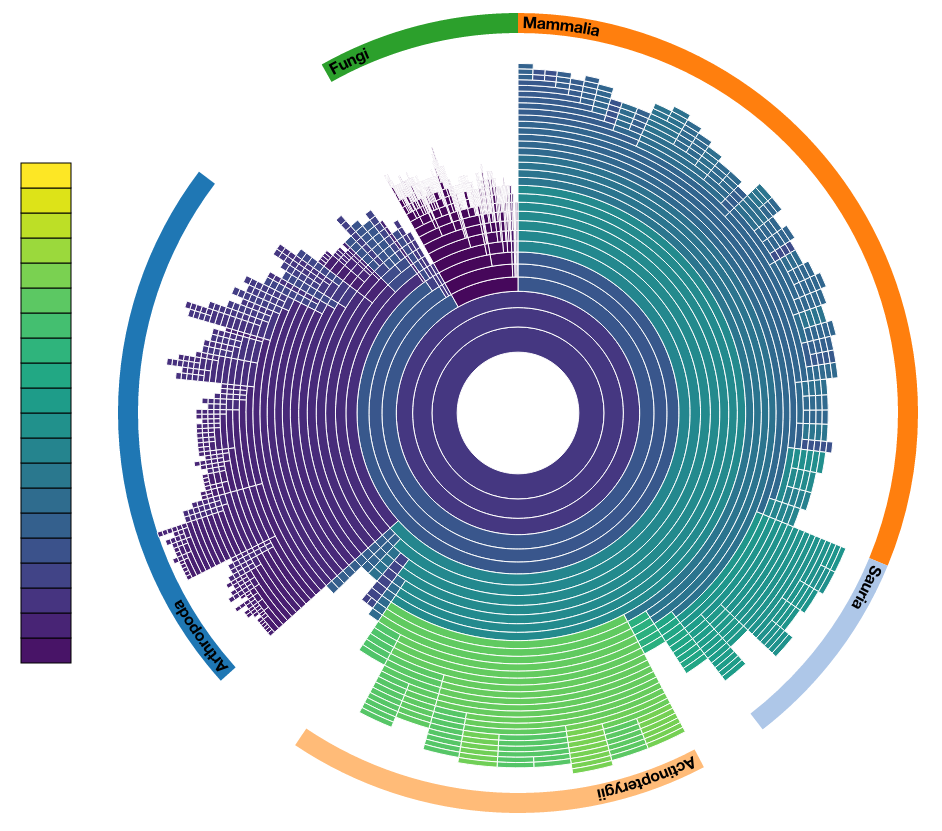
\includegraphics[width=.8\textwidth]{Seriola_lalandi}
\end{figure}

Figure~\ref{fig:seriola} shows the result from a ray-finned fish,  \textit{Seriola lalanda}. This is a good sanity check: the \textit{Actinopterygii} 
group is well-scored, as we would expect given the species evolutionary history. Other more closely-related metazoans also have
moderate scores, and the Arthropods and Fungi score very poorly.

\begin{figure}[!ht]

  \caption{Result generated from the Chickadee transcriptome. While \textit{Sauria} scores highly here, most of the non-Arthropod
  				 metazoans score do too.}\label{fig:chick}
  \centering
    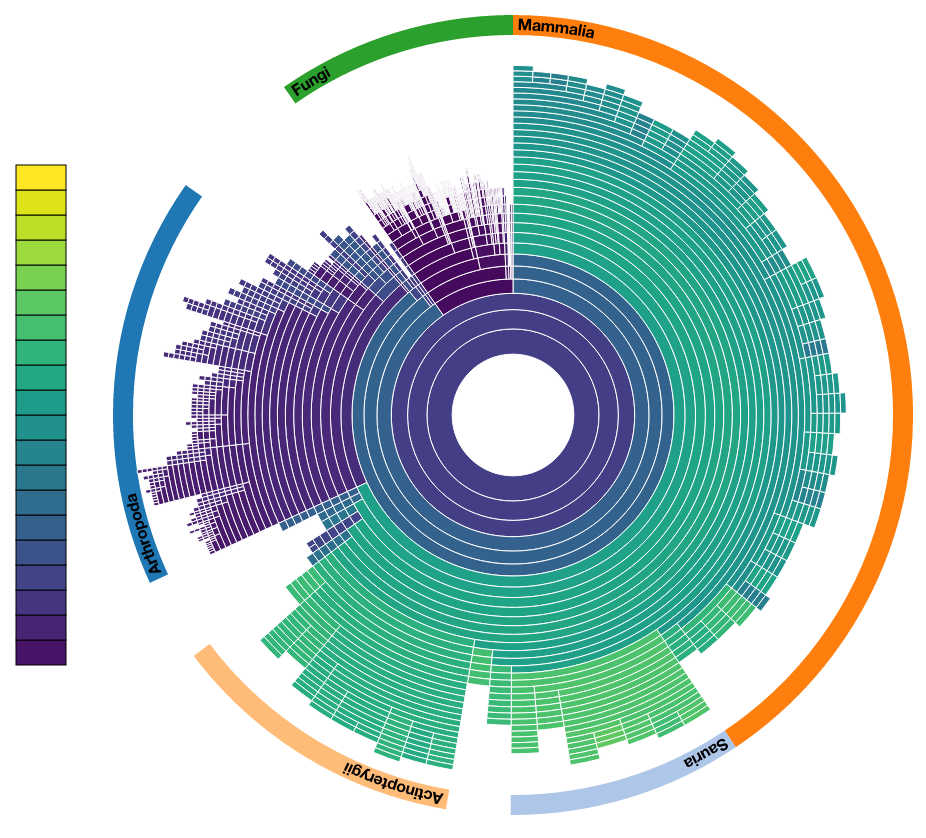
\includegraphics[width=0.8\textwidth]{Chickadee}
\end{figure}

Figure~\ref{fig:chick} also shows this view. This one came from the Chickadee, a common bird. While not as tight as the \textit{Seriola lalanda}
result, it still matches expectations.

\begin{figure}[!ht]
  \caption{Full \textit{explotiv} window with  \textit{Petromyzon marinus}, ie sea lamprey. This demonstrates clade
  				selection (the dark wedge at 6 o'clock) score distribution histogram for the selected species. This low-scoring 
  				result is rather disappointing, considering that I produced this particular transcriptome assembly myself!}\label{fig:pmar}
  \centering
    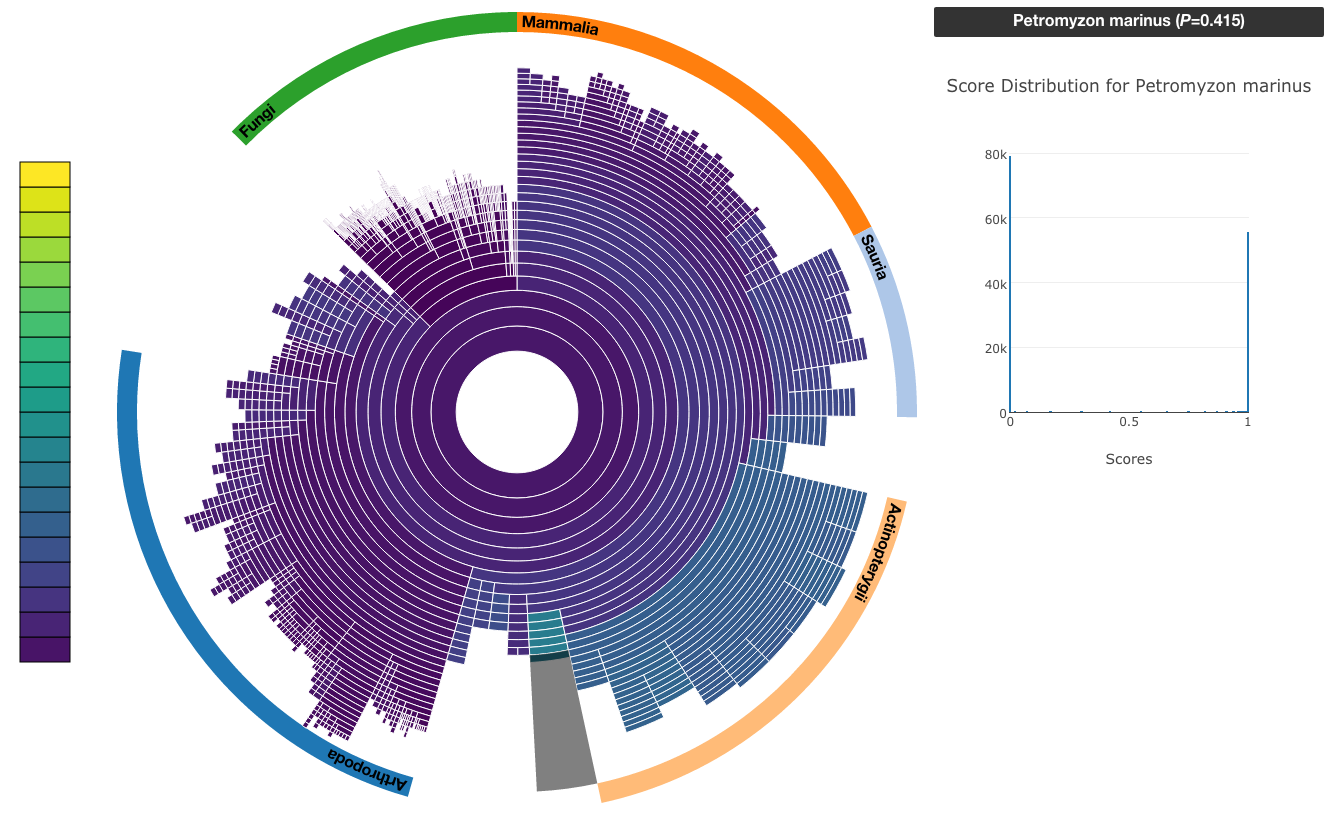
\includegraphics[width=0.8\textwidth]{p_marinus}
\end{figure}

In Figure~\ref{fig:pmar}, we are shown the complete \textit{explotiv} window from \textit{Petromyzon marinus} data. There is an active selection on the \textit{Petromyzon marinus} node,
and a corresponding score distribution histogram on the right. This particular histogram is heavily biased to high scores, as the species itself
is represented in this database. Unfortunately, this is a poor result -- almost all nodes are low probability, and even the \textit{Petromyzon marinus}
node only reaches 0.415. However, this is not due to \textit{explotiv}; I assembled this transcriptome myself as a part of a different research project,
and this figure serves to confirm other data that the assembly result was mediocre, and possibly even contaminated.

\section{Discussion}

Overall, the \textit{explotiv} phylogenetic view seems to give pleasing results. However, there is significant future work to be done. Some of this
work is in small details: more labels are needed (such as text for the color bar legend), several portions of the sunburst could use group annotations
(the nematodes would be good to add), and species data should be parsed from an external API (\url{mygene.info} is the planned target). The more
important work is expanding the database resource: OrthoDB, while a good starting point, is limited, with no bacteria and only a small subset of
eukaryotes. The next challenge then will be converting the implementation to use SwissProt, which is much more comprehensive and will allow
more useful analyses; including bacteria, for example, will make \textit{explotiv} a powerful tool for immediately identifying contamination, an
ongoing problem with all RNA-seq analyses.

Additionally, the original plan for this project called for an annotation explorer integrated with dammit. While progress was made on that front,
due to time constraints, effort was switched over to the \textit{explotiv} viewer. Eventually, \textit{explotiv} will be shipped as a submodule
of dammit (hence the name!), and will link directly from the summary view to the results of dammit's annotations. For now though, it only
makes use of dammit to generate alignments and provide some data access, leaving the messier parts of the integration for a later project.

\bibliographystyle{ieeetr}
\setcitestyle{numbers, open={[},close={]}}
\bibliography{explotiv}

\end{document}
